\section{Results}
\label{sec:results}

\subsection{The hybrid does not improve accuracy}
\label{sec:no-accuracy-gain}

Table~\ref{tab:fusion-variants} reports every decision variant for the focused
backbone and Fig.~\ref{fig:results}(a) plots the same ordering. The AI alone reaches
0.6575 macro-F1 and 0.8762 accuracy; the primary
per-channel hybrid reaches 0.6602 and 0.8774, a gain of 0.0027 macro-F1 and eight
additional correct comments (5{,}861 versus 5{,}853). The gain is concentrated in
\hate{}: F1 rises from 0.5830 to 0.5906, driven by recall (0.5334 to 0.5494) at a
small cost in precision (0.6427 to 0.6385). \off{} and \clean{} do not pay for it
(0.4493 to 0.4494, 0.9403 to 0.9407): the change is an extension of \hate{} recall,
not a reallocation between classes.

The other variants locate the effect: per-channel weights add 0.0010 macro-F1 over
a single global weight (0.6583 to 0.6593) and thresholds a further 0.0009. The
logistic meta-classifier is \emph{worse} than the AI alone (0.6513): fitting six
features on 2{,}672 validation comments overfits the rule scores and shifts the
operating point towards \hate{} recall. Thresholds do make the rule engine usable
on its own---0.5258 macro-F1, identical standalone and inside the pipeline, against
0.4714 with argmax, which collapses on \off{}---but it stays far below the
transformer (0.8421 accuracy).

\begin{table}[ht]
\centering
\scriptsize
\setlength{\tabcolsep}{3pt}
\caption{Decision-level variants for the focused backbone
(\model{sensitiveai-vi-custom}) on the test split. Every variant reads the same
frozen scores; only the mixing and decision rule differ. The last row is the
paper's primary system. \emph{Per-class columns are F1}; the best macro-F1 is
in bold. The two rule-only rows
are scored inside the fusion pipeline on the renormalised rule scores; the
standalone rule engine, with its own thresholds, is reported in the text.}
\label{tab:fusion-variants}
\begin{tabular}{lccccc}
\toprule
System & Acc. & Macro-F1 & \hate & \off & \clean \\
\midrule
AI only (argmax)                      & 0.8762 & 0.6575 & 0.5830 & 0.4493 & 0.9403 \\
Rule only (argmax)                    & 0.8494 & 0.4714 & 0.4867 & 0.0000 & 0.9274 \\
Rule only (frozen thresholds)         & 0.8421 & 0.5258 & 0.4102 & 0.2389 & 0.9284 \\
\midrule
Fusion, global $\alpha$ (argmax)      & 0.8769 & 0.6583 & 0.5851 & 0.4490 & 0.9408 \\
Fusion, global $\alpha$ (thresholds)  & 0.8769 & 0.6583 & 0.5851 & 0.4490 & 0.9408 \\
Fusion, logistic meta-classifier      & 0.8626 & 0.6513 & 0.5818 & 0.4379 & 0.9341 \\
Fusion, per-channel $\alpha$ (argmax) & 0.8774 & 0.6593 & 0.5882 & 0.4488 & 0.9408 \\
Fusion, per-channel (thresholds)      & 0.8774 & \textbf{0.6602} & 0.5906 & 0.4494 & 0.9407 \\
\bottomrule
\end{tabular}
\end{table}


\begin{figure}[ht]
\centering
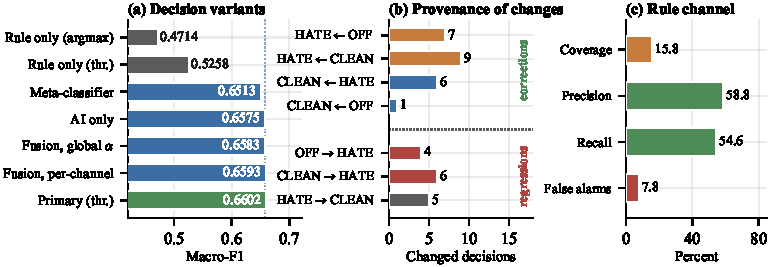
\includegraphics[width=\textwidth]{figures/results.pdf}
\caption{Quantitative summary for the focused backbone. (a)~Macro-F1 of every
decision variant; the dotted line is AI-only and the green bar is the primary
system. (b)~Provenance of the 38 changed decisions: the four correction types and
the three regression types. (c)~Behaviour of the rule
channel on the test split: coverage, precision when firing, recall on non-\clean{}
comments, and false alarms on \clean{}. Values are percentages; raw counts are in
the text and in panel~(b).}
\label{fig:results}
\end{figure}

\subsection{The difference is not distinguishable from zero}
\label{sec:significance-results}

Table~\ref{tab:backbones} makes the negative result explicit. For the focused
backbone the paired-bootstrap difference is $-0.0027$ with a 95\% interval of
$[-0.0079,+0.0027]$ and $p=0.29$; McNemar on the 38 changed decisions gives $b=15$,
$c=23$, $p=0.26$. Across the four backbones every bootstrap interval contains zero.
Where McNemar does reach significance the sign flips: the standard-head backbone
loses 61 comments to the hybrid and wins back 30 ($p=0.0015$), while the curriculum
backbone loses 8 and wins back 31 ($p=0.0003$). Fusion therefore helps one recipe and
hurts another by margins the aggregate macro-F1 cannot separate. We do not claim an
accuracy improvement: the hybrid is \emph{accuracy-neutral}, changing 38 decisions
without moving the aggregate metric beyond noise.

\subsection{The rule channel is narrow and precise-ish}
\label{sec:rule-channel-results}

The rule engine fires on 1{,}052 of 6{,}680 comments (15.75\%), not on the majority
of the test set. When it fires, 58.75\% of the comments are truly non-\clean{}, so
roughly two in five firings are false alarms; it recovers 54.59\% of non-\clean{}
comments and fires on 7.82\% of \clean{} comments (Fig.~\ref{fig:results}c). It is
useful as evidence, not as a decision: silent on 45\% of toxic comments and wrong
about a substantial share of those it flags. Coverage is low by construction---most
entries are multi-word, context-required phrases and validation zeroed the
accent-less alias weight---so the channel matches near-canonical forms rather than
respellings: narrow and inspectable rather than broad and opaque.
